% ============================================================
%  Section 9: Epistemic Uncertainty Analysis
%  H&E to Sirius Red Virtual Staining Paper
% ============================================================

\section{Epistemic Uncertainty Analysis}
\label{sec:uncertainty}

The scaling study~(Section~\ref{sec:results_scaling}) characterises translation quality
for each configuration but treats each as a deterministic predictor.
In an unpaired setting no paired SR target supervises the generator, so a model may
produce a stain that appears plausible yet does not reproduce the underlying tissue
structure, and without ground truth such errors cannot be detected per tile.
We can, however, train independently seeded models and ask whether they converge on the
same translation.
To this end, we train deep ensembles of $K{=}10$ independently seeded models per family
and treat the pixel-wise variance across ensemble members as an epistemic uncertainty
signal: low variance indicates the unsupervised objective steers all members toward a
common SR output, while persistent inter-seed disagreement marks inputs where the
objective alone does not pin down a unique answer.
Variance measures epistemic uncertainty, not correctness, and must be read alongside
CPA~MAE from the scaling study: a model can be confidently wrong.

\begin{figure*}[t!]
  \centering
  \setlength{\tabcolsep}{2pt}
  \renewcommand{\arraystretch}{0.4}
  \small
  \begin{tabular}{lcccc}
     & \textbf{H\&E input} & \textbf{Real SR} & \textbf{CycleGAN-M$\times$100\%} & \textbf{CycleDiff-S$\times$25\%} \\[1pt]
    \textbf{Patch 1} &
    \includegraphics[width=0.20\linewidth]{images/visualize/1_1.png} &
    \includegraphics[width=0.20\linewidth]{images/visualize/1_2.png} &
    \includegraphics[width=0.20\linewidth]{images/visualize/1_3.png} &
    \includegraphics[width=0.20\linewidth]{images/visualize/1_4.png} \\
    % Tile 1, mask &
    & &
    \includegraphics[width=0.20\linewidth]{images/visualize/2_2.png} &
    \includegraphics[width=0.20\linewidth]{images/visualize/2_3.png} &
    \includegraphics[width=0.20\linewidth]{images/visualize/2_4.png} \\[4pt]
    \textbf{Patch 2} &
    \includegraphics[width=0.20\linewidth]{images/visualize/3_1.png} &
    \includegraphics[width=0.20\linewidth]{images/visualize/3_2.png} &
    \includegraphics[width=0.20\linewidth]{images/visualize/3_3.png} &
    \includegraphics[width=0.20\linewidth]{images/visualize/3_4.png} \\
    % Tile 2, mask &
    & &
    \includegraphics[width=0.20\linewidth]{images/visualize/4_2.png} &
    \includegraphics[width=0.20\linewidth]{images/visualize/4_3.png} &
    \includegraphics[width=0.20\linewidth]{images/visualize/4_4.png} \\
  \end{tabular}
  \caption{%
    Qualitative comparison on two held-out H\&E patches. For each patch, the top row
    shows the H\&E input, the loosely registered real Sirius Red ground truth, and the
    virtual SR produced by CycleGAN's medium generator at 100\% training data and
    CycleDiffusion's small generator at 25\% training data. The bottom row shows the
    nnU-Net~v2 collagen segmentation masks of the corresponding real and virtual SR
    images, from which CPA is computed. Because the H\&E and SR sections are
    non-adjacent cuts, visible differences between the real and virtual SR images
    reflect both true translation error and irreducible inter-section variation.
    These two configurations bracket the study: the CycleGAN-M 100\% configuration
    records the study-best CPA~MAE across all 54 configurations, while the
    CycleDiffusion-S 25\% configuration records the study-worst.%
  }
  \label{fig:qualitative_examples}
\end{figure*}


\noindent\textbf{Model selection.}
For each family we select the generator size trained on the full training set (100\%
data fraction) with the lowest CPA~MAE (FID as tiebreak), marked with a star
($\bigstar$) in Figure~\ref{fig:results_overview} and listed in
Table~\ref{tab:best_per_family}.

\noindent\textbf{Ensemble training.}
We use deep ensembles rather than MC~dropout: a calibration study of unpaired image
translation found MC~dropout poorly calibrated in this regime, while deep ensembles
yield well-calibrated estimates with minimal
tuning~\cite{trustworthy_i2i2025, lakshminarayanan2017simple}.
Each selected configuration is re-trained ten times with distinct random seeds;
hyperparameters and training data match the corresponding scaling-study run.
The ensemble size of $K{=}10$ matches convergence analyses showing that calibration
errors and mean epistemic uncertainty both plateau near ten members for biomedical image
segmentation~\cite{siddiqui2024uncertainty} and prior ensemble-based virtual staining
work~\cite{insilicolabeling2023}; additional members yield diminishing returns
at substantial compute cost, as each member requires a full retraining of the
underlying model.

% -------------------------------------------------------
\subsection{Uncertainty Quantification}
\label{sec:uncertainty_quantification}
% -------------------------------------------------------

For each selected configuration, given an H\&E input $x$ and the $K{=}10$
independently trained generators $\{G_k\}_{k=1}^{K}$ (schematic in \suppsec{5}), the ensemble mean is the pixel-wise average
$\bar{y}(x) = \frac{1}{K}\sum_{k} G_k(x)$, and the epistemic uncertainty map
$\mathbf{U}(x) \in \mathbb{R}^{H \times W}$ is the sum of per-channel sample variances
across ensemble members~\cite{lakshminarayanan2017simple}:
\begin{equation}
  \mathbf{U}(x) = \sum_{c=1}^{C} \frac{1}{K-1}
  \sum_{k=1}^{K} \bigl(G_k(x)_{c} - \bar{y}(x)_{c}\bigr)^{2},
  \label{eq:uncertainty}
\end{equation}
where $C{=}3$ is the number of output channels (RGB).
Summing channels preserves the total disagreement signal; high values of
$\mathbf{U}(x)$ flag regions where the model fails to converge on a consistent
translation across seeds, i.e., the inter-seed disagreement signal motivated above.
A per-tile summary is the spatial mean standard deviation
$\bar{\sigma}(x) = \frac{1}{|\mathcal{T}|}\sum_{p \in \mathcal{T}} \sqrt{\mathbf{U}(x)_p}$
over tissue pixels $\mathcal{T}$, used as the per-family epistemic uncertainty
statistic summarised in Figure~\ref{fig:uncertainty_boxplot}.

% -------------------------------------------------------
\subsection{Results: Ensemble Variance}
\label{sec:unc_variance_results}
% -------------------------------------------------------

\begin{figure*}[t!]
  \centering
  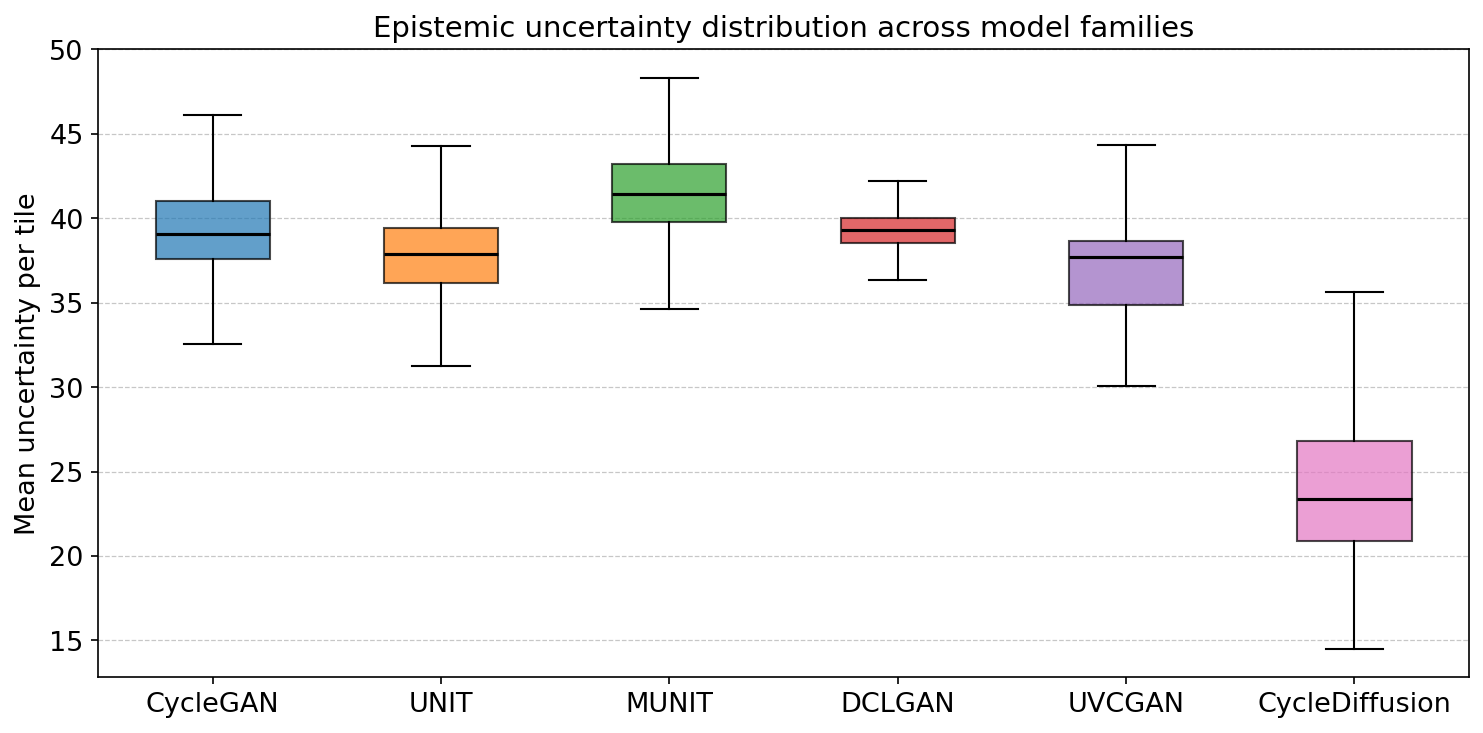
\includegraphics[width=0.85\linewidth]{images/uncertainty_boxplot}
  \caption{%
    Distribution of per-tile epistemic uncertainty $\bar{\sigma}$ across $9{,}365$
    test tiles (those with at least $0.1\%$ tissue mask coverage) for each of the six
    model families; median values are annotated.
    GAN-based families cluster within a narrow band (median $37.68$--$41.42$,
    IQR $1.48$--$3.80$); CycleDiffusion sits below the cluster (median $23.35$) yet
    shows substantially wider spread (IQR $5.89$).%
  }
  \label{fig:uncertainty_boxplot}
\end{figure*}

Figure~\ref{fig:uncertainty_boxplot} reports the per-tile $\bar{\sigma}$ distribution
across the $9{,}365$ test tiles for each model family.
The reported values are spatial-mean standard deviations summed across the three
RGB channels on the $0$--$255$ intensity scale, so a per-tile value of ${\sim}39$
corresponds to roughly $13$ intensity units per channel (${\sim}5\%$ of the full
range).

\paragraph{GAN families.}
The five GAN-based methods cluster within a narrow uncertainty band, with medians
ranging from $37.68$ (UVCGAN) to $41.42$ (MUNIT) and IQRs of $3.26$--$3.80$.
DCLGAN is the exception within this group: its median ($39.29$) is comparable to the
other GAN families, yet its IQR ($1.48$) is approximately half that of any other GAN
family.
MUNIT records the highest median ($41.42$) among GAN families.

\noindent\textbf{CycleDiffusion.}
CycleDiffusion sits distinctly below the GAN cluster in typical uncertainty (median
$23.35$), yet its IQR ($5.89$) is $1.6$--$4\times$ wider than any GAN family.
On many tiles the ten independently seeded diffusion models converge on a consistent
SR translation, while on a substantial subset they diverge sharply, a tile-level
variability absent in all GAN families.

\noindent\textbf{Joint reading with CPA~MAE.}
Combined with the CPA~MAE values of Section~\ref{sec:results_scaling}, the two axes
separate the families: CycleGAN's medium generator pairs the study-low CPA~MAE
($0.008 \pm 0.007$) with moderate uncertainty (median $39.09$, IQR $3.39$), DCLGAN pairs
low CPA~MAE ($0.028$) with the narrowest spread (IQR $1.48$), and CycleDiffusion pairs
moderate CPA~MAE ($0.051$) with the lowest median but widest spread.
UNIT, MUNIT, and UVCGAN occupy intermediate positions on both axes.

A complementary calibration analysis against cycle-reconstruction error
(\suppsec{5}) shows that GAN-based uncertainty maps moderately predict
tile-level error (across-tile Pearson $\rho = 0.50$--$0.66$), with DCLGAN
($\rho = 0.66$, ECE $0.055$) and MUNIT ($\rho = 0.62$, ECE $0.058$) leading.
CycleDiffusion's uncertainty is uncorrelated with cycle error ($\rho = {-}0.03$),
and no family achieves meaningful within-tile spatial calibration.

% ============================================================
%  New bibliography entries for this section
%  (merge with references.bib)
% ============================================================
%
% @article{trustworthy_cell_ensemble2023,
%   author  = {Rauber, Paul and others},
%   title   = {Trustworthy in silico cell labeling via ensemble-based image translation},
%   journal = {Nature Communications},
%   year    = {2023},
%   note    = {PMC10663640},
%   url     = {https://pmc.ncbi.nlm.nih.gov/articles/PMC10663640/}
% }
%
% (Shared entries already listed:
%  lakshminarayanan2017simple, gal2016dropout, trustworthy_i2i2025)
